\begin{figure}[H]
\centering
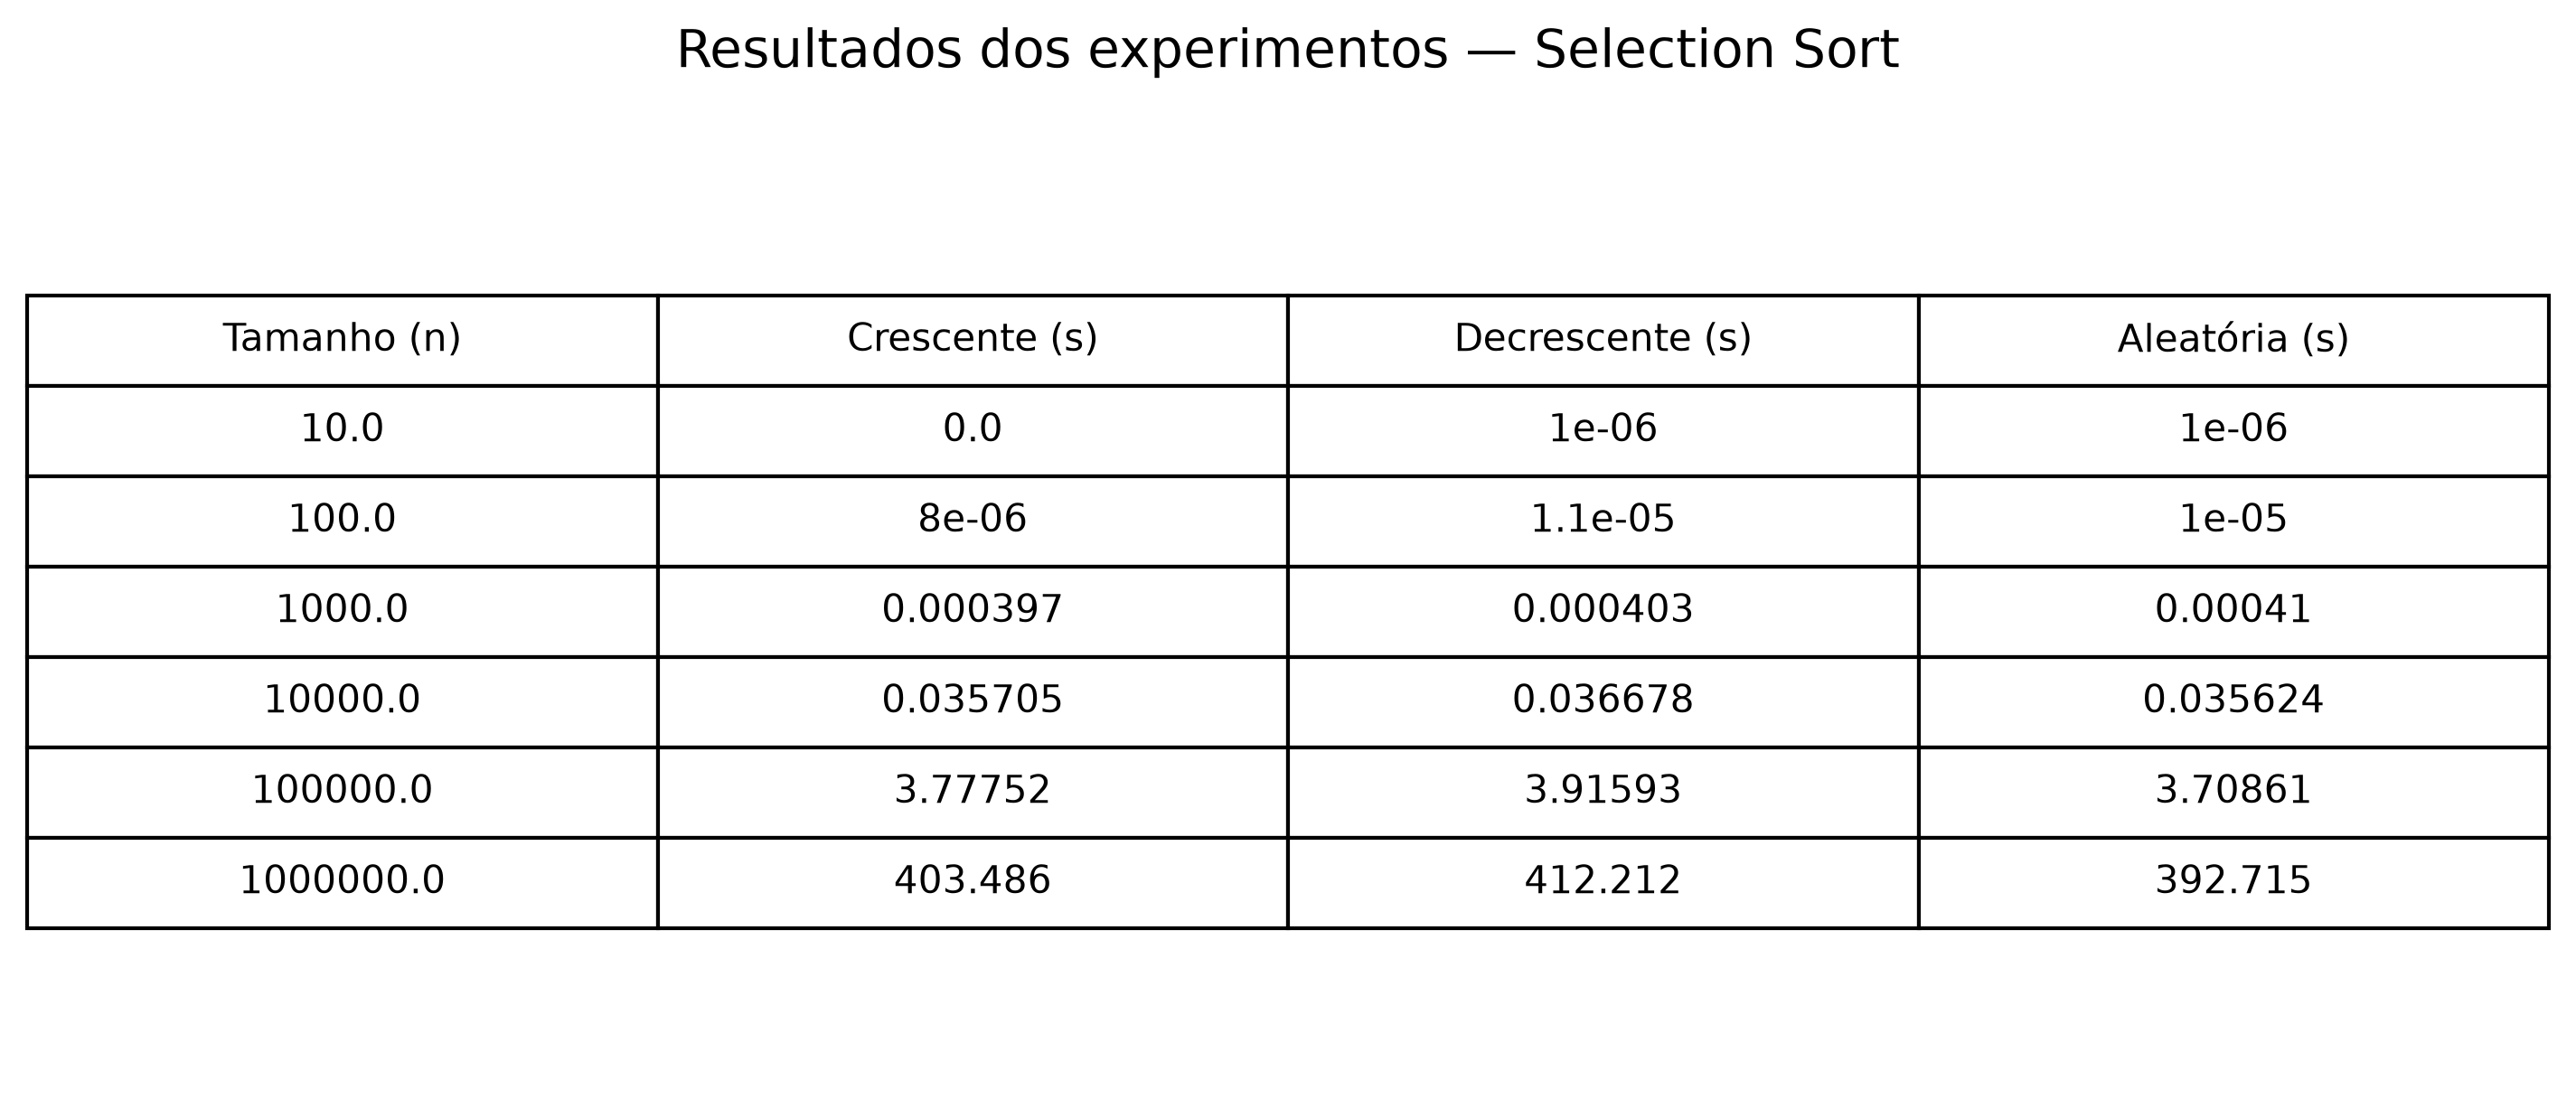
\includegraphics[width=16cm]{Imagens/Selection_Sort/tabela.png}
\caption{Tabela de tempo de execução do algoritmo Selection Sort}
\label{fig:tabela-selection}
\end{figure}

\begin{figure}[H]
\centering
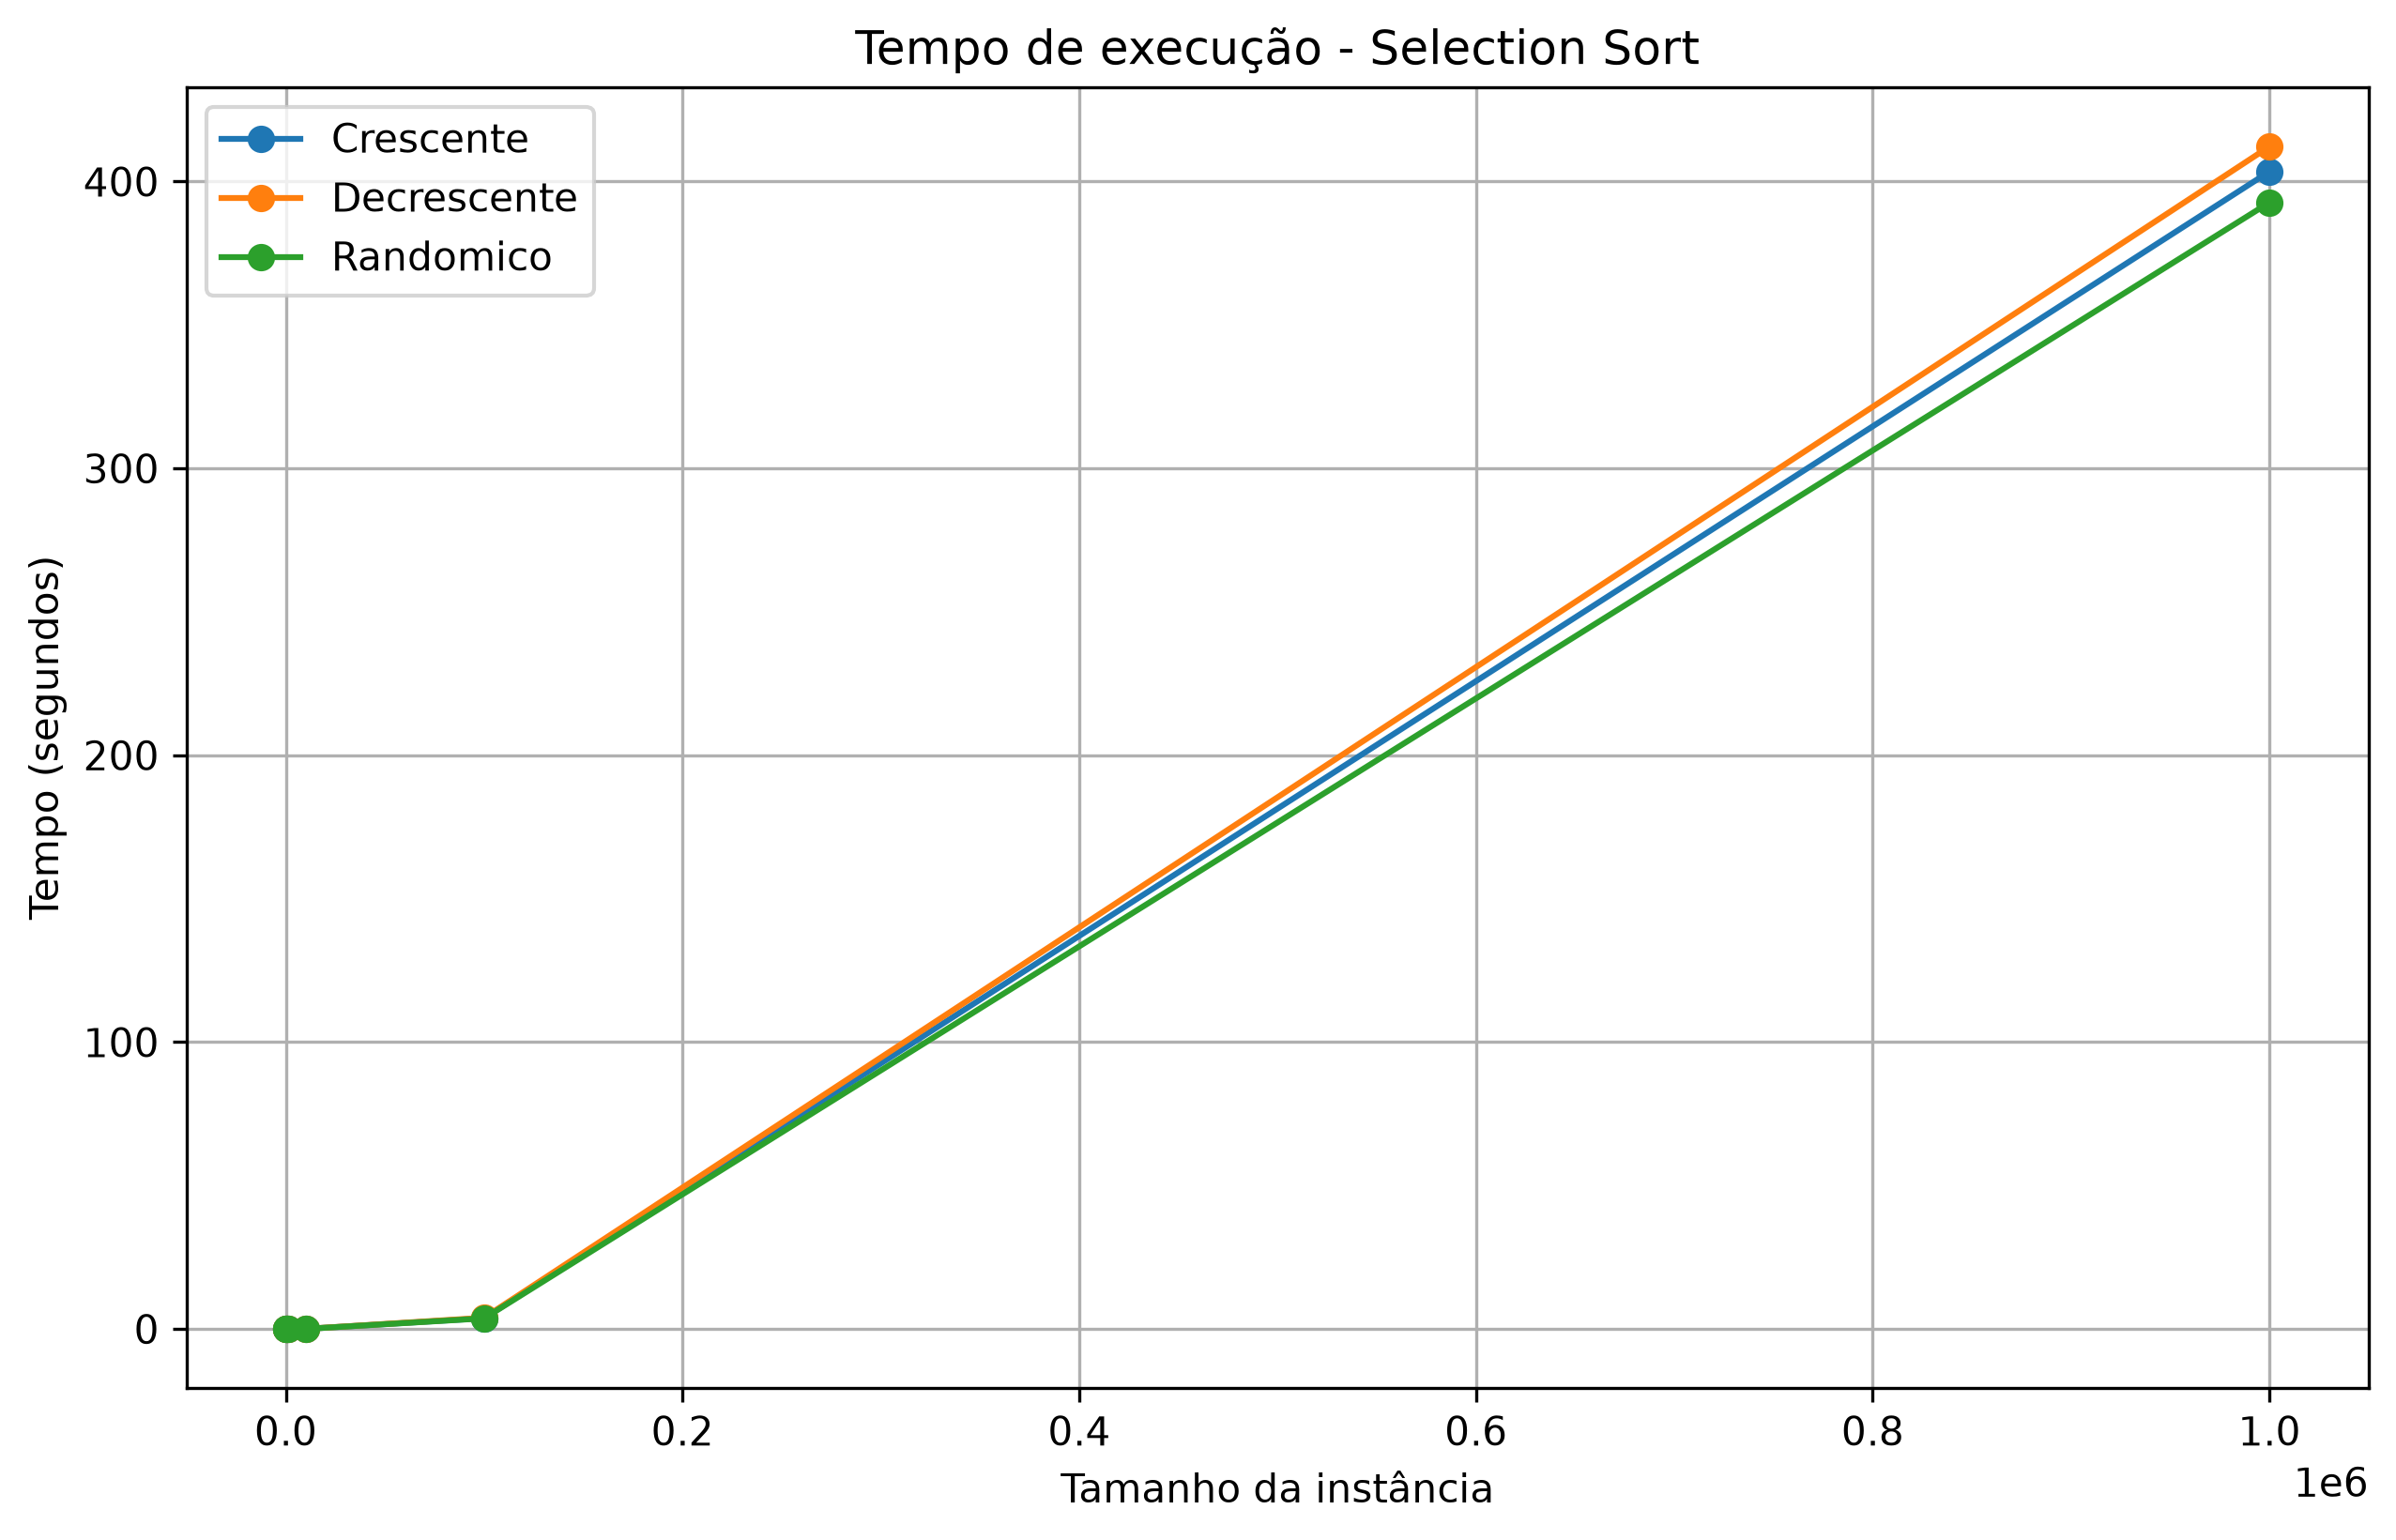
\includegraphics[width=10cm]{Imagens/Selection_Sort/grafico.png}
\caption{Gráfico de tempo de execução do algoritmo Selection Sort}
\label{fig:grafico-selection}
\end{figure}

Os resultados obtidos nos experimentos estão apresentados na tabela e no
gráfico. Observa-se que o algoritmo Selection Sort apresenta comportamento
semelhante nos diferentes tipos de entrada, pois a quantidade de
comparações realizadas não depende da organização inicial dos elementos.

Nas instâncias ordenadas de forma crescente, o algoritmo ainda precisa
percorrer a parte não ordenada do vetor para encontrar o menor elemento.
Dessa forma, mesmo quando os elementos já estão organizados, são
realizadas aproximadamente as mesmas comparações previstas para os demais
tipos de entrada.

Nas instâncias ordenadas de forma decrescente, o algoritmo também realiza
a mesma quantidade de comparações, embora a posição do menor elemento
encontrado possa exigir mais trocas para colocá-lo na posição correta.

As instâncias aleatórias apresentam comportamento semelhante, pois,
independentemente da disposição inicial dos elementos, o algoritmo
continua procurando o menor elemento em toda a parte ainda não ordenada
do vetor.

A partir dos dados, também é possível perceber que o aumento do tamanho
da entrada provoca um crescimento significativo no tempo de execução.
Esse comportamento está de acordo com a análise teórica, segundo a qual
o Selection Sort apresenta complexidade $\Theta(n^2)$ no melhor caso,
caso médio e pior caso.

Assim, os resultados experimentais apresentam comportamento compatível
com a análise de complexidade do algoritmo Selection Sort.
